\section{Results}
\textcolor{blue}{Speaking about the three methods on with tweet-embeddings}

As the two convolutional neural nets were giving the best results, they were trained for longer times using the full dataset provided. After a few hours of training, some results appeared [FIG. \ref{plot:CNNaccuracy}]. The figure display the training accuracy of the two models. The first one was not using the dropout method as opposed as the second one. Each time the whole dataset was trained  



\label{sec:results}
\begin{figure}[h!]
\centering
	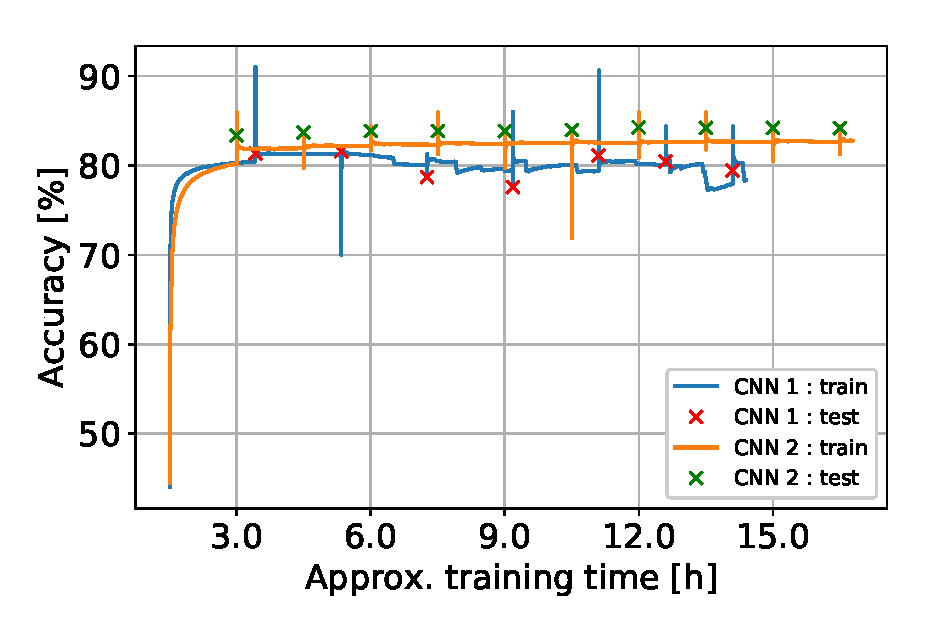
\includegraphics[scale=0.6]{CNNaccuracy} 
\caption{Training of the two convolutional neural nets. The first one does not use ``dropout'' as opposed as the second one.}
\label{plot:CNNaccuracy}
\end{figure}
\FloatBarrier


\begin{table}[h]
  \centering
  \begin{tabular}[c]{lllll}
    Input format&Model&Precision&Recall&Accuracy\\
    \hline
    Tweet-embed.&Logistic regression &    60.84   & 60.64 & 60.60 \\
    Tweet-embed.&SVM                 &   63.69     & 62.05  & 61.96 \\
    Tweet-embed.&Neural network	& 66.47	& 65.88	& 65.83 \\
    Word-embed.&CNN w.o. dropout   & 0.00	& 0.00	&  81.12 \\
    Word-embed.&CNN w. dropout & 0.00 & 0.00 & 84.21
    
  \end{tabular}
  \caption{Classification performances using local hold-out testing, for various input data formats.All the data are given in \%}
  \label{tab:results}
\end{table}


